\documentclass{article}
\usepackage[utf8]{inputenc}
\usepackage[margin=0.75in]{geometry}
\usepackage{cite}
\usepackage{colortbl}
\usepackage{booktabs}% http://ctan.org/pkg/booktabs
\newcommand{\tabitem}{~~\llap{\textbullet}~~}
\usepackage[hidelinks]{hyperref}
\usepackage{subcaption}
\usepackage{graphicx}
\usepackage{titlesec}% http://ctan.org/pkg/titlesec
\titleformat{\section}%
    [hang]% <shape>
    {\normalfont\bfseries\Large}% <format>
    {}% <label>
    {0pt}% <sep>
    {}% <before code>
\renewcommand{\thesection}{}% Remove section references...
\renewcommand{\thesection}{\arabic{section}}
% \renewcommand{\thesubsection}{\arabic{subsection}}%... from subsections
\usepackage{bookmark}
\usepackage{enumitem}
\usepackage{multicol}
\usepackage{mathtools}
\usepackage{lipsum}  
\setcounter{secnumdepth}{3} % default value for 'report' class is "2"


\DeclarePairedDelimiter{\ceil}{\lceil}{\rceil}
\usepackage[figuresleft]{rotating}

\begin{document}
\begin{center}

    % MAKE SURE YOU TAKE OUT THE SQUARE BRACKETS

    \LARGE{\textbf{COMP 3004 - Deliverable \#3 \\ System Architecture and Design}}\\ 
    % \vspace{1em}
    \Large{\href{https://github.com/alextrosta/brackit}{\texttt{Brackit}} - Mobile Tournament Bracket Creation} 
    % \vspace{1em}
    % \normalsize\textbf{Jaime Herzog, Suohong Liu, Xiyi Liu, Alex Trostanovsky} \\
    % \normalsize{
    %     \href{mailto:jaime.herzog@carleton.ca}{jaime.herzog@carleton.ca},
    %     \href{mailto:suohong.liu@carleton.ca}{suohong.liu@carleton.ca},
    %     \href{mailto:xiyi.liu@carleton.ca}{xiyi.liu@carleton.ca},
    %     \href{mailto:alex.trostanovsky@carleton.ca}{alex.trostanovsky@carleton.ca}
    % }\\
    % \normalsize{
    %     101009321,
    %     101002340,
    %     101004577,
    %     100984702,
    % }
    % \vspace{1em}
    % \normalsize{Carleton University, School of Computer Science} \\
\end{center}
% \begin{normalsize}

% \end{normalsize}

\section*{Metadata}
\subsection*{Team / App Name: \href{https://github.com/alextrosta/brackit}{\texttt{Brackit}}}
% \textbf{Team Member Names:}\\ Jaime Herzog: 101009321, Suohong Liu: 101002340, Xiyi Liu: 101004577, Alex Trostanovsky: 100984702


\subsection*{Team member names}
\begin{center}
    \begin{tabular}{ |l|c| }
        \hline
        \textbf{Name}     & \textbf{Student ID} \\
        \hline
        Jaime Herzog      & 101009321           \\
        Suohong Liu       & 101002340           \\
        Xiyi Liu          & 101004577           \\
        Alex Trostanovsky & 100984702           \\
        \hline
    \end{tabular}
\end{center}
\tableofcontents

\clearpage
\section{Architecture}
% identify, describe, and justify the architecture of your project (architectural style, design patterns) \\
% Outcome is a system architecture that supports the functional goals and non-functional attributes of your project 
\subsection{Description}
\subsubsection{Functional \& Non-Functional Requirements}
\texttt{Brackit} addresses an urgent need by tournament organizers and attendants to visualize, manage, and interact with double elimination
brackets on their mobile devices. At a high level, we committed to developing a product that will meet the following \textbf{functional requirements}:
\begin{enumerate}
    \item{Tournament Organizers (TO's) can create, host, maintain, and visualize double elimination brackets.}
    \item{Registered \texttt{Brackit} Users, as well as Guests, can use the application to join created tournaments.}
    \item{\texttt{Brackit} will store and maintain user profiles that will describe users' past performance. For example:
    \begin{itemize}
        \item{Matches won/lost}
        \item{Tournaments entered/created}
    \end{itemize}
    }
\end{enumerate}
In terms of \textbf{non-functional requirements}, we believed \texttt{Brackit} should be \textit{usable} on mobile devices. \texttt{Brackit} users should be able to:
\begin{itemize}
    \item{View and access all components (Brackets, Rounds, Matches) of a tournament on an Android device.}
    \item{Seamlessly enter tournament competitors to brackets on an Android device.}
\end{itemize}
% \subsubsection{Components and Connectors}
Conceptually, \texttt{Brackit} needed to support the creation and maintenance of the following \textit{components}:
\begin{itemize}
    \item{\textit{Tournament}: The highest level of abstraction utilized in Bracket creation. A tournament acts as a \textit{container} for brackets. \texttt{Brackit} supports double-elimination tournaments, where competitors cease to be eligible to win the tournament after losing two matches \cite{wiki:det}.}
    \item{\textit{Bracket}: Given the number of entrants and their corresponding seeds (ranks), 
    Double elimination brackets dictate competitor matchups and the progression of competitors through the Winners and Losers brackets. 
    Brackets contain 
    a dynamic list of Rounds. }
    \item{\textit{Round}: Rounds contain a dynamic list of Matches.}
    \item{\textit{Match}: Matches pair the strongest and corresponding weakest players in a Round according to rank. (That is, in a tournament containing $n$ players, the top (1\textsuperscript{st}) ranked player will be matched with the lowest ($n-1$) ranked player, the 2\textsuperscript{nd} ranked player will be matched with the $n-2$ ranked player, etc.)}
\end{itemize}  
% To develop the interface between each of the components mentioned above, we decided to implement the following \textit{connectors}:
% \begin{itemize}
%     \item{}
    
% \end{itemize}
\subsection{Justification of Architectural Style Choices}
\subsubsection{Object-Oriented Architectural Style}
\label{sssec:ooas}
As described above, a Double Elimination Tournament mobile management application must maintain a set of well-defined entities (i.e. Tournaments, Brackets, Rounds, and Matches) with predetermined relationships. For example, given $n$ competitors, a correct double-elimination tournament will contain $\ceil{\lg n}$ rounds in the Winners bracket and $\ceil{\lg n} + 
\ceil{\lg \lg n}$ rounds in the Losers bracket \cite{de_formula}. Also, the progression of competitors can be calculated at the creation of a tournament, and handling this progression follows a deterministic approach (e.g. The winner of Match 1 of Round 1 in the Winners Bracket will always progress to Match 1 Round 2 in the Winners Bracket - see Figure \ref{fig:deb} for an illustrative example).\\
Therefore, to encourage an efficient decomposition of the algorithm and entities associated with Double Elimination Tournament management, we decided to model the architecture of \texttt{Brackit} using an \textbf{Object-Oriented} (OO) architecture. 
Specifically, we chose to model each of the components of our application as objects. This allowed us to encapsulate the expected behaviour of each of the tournament objects while maintaining a valid separation of concerns. To explicate the validity of the choice of an OO architecture for \texttt{Brackit}, consider the dynamic nature of Tournament creation.\\
A tournament bracket acts as a container for rounds, which themselves act as containers for matches.
To handle tournament progression, the data associated with each match (i.e. which competitor won or lost) should be self-contained within the match object instantiation, but also must be accessible through attributes of that object. Defining the Match construct as an object enables self-contained class methods and attributes that achieve these intended behaviours. At the same time, setting the Win / Loss attribute of a match as publicly visible allowed us to develop querying strategies that can provide score summaries for participating users. 
    \begin{figure}[htp]
        \centering
        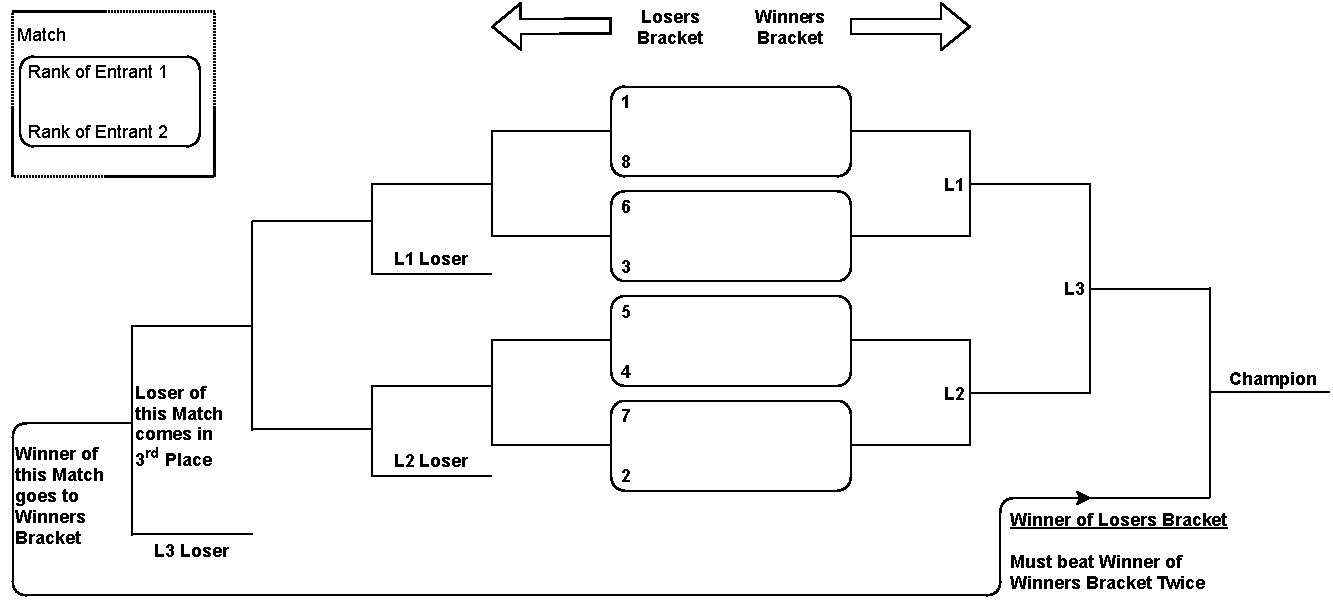
\includegraphics[width=12cm]{../diagrams/double_elim_bracket_comp.pdf}
        \caption{Seeded Double Elimination Tournament Chart for 8 competitors. (Adapted from \cite{se:tba})}
        \label{fig:deb}
        \end{figure}
\subsubsection{Client-Server Architectural Style}
A \textbf{Client-Server} architecture dictates that a server host, deliver, and manage most of the resources and services that clients can consume. Client-server architectures are used in situations where separation of concerns exists between the client and the server. The modularity inherent in this style lends itself to the development of scalable software \cite{sa_waterloo}. \\
We decided to follow the guidelines set out by the Client-Server Architectural Style because we believed \texttt{Brackit} should provide the following core features: Double Elimination bracket algorithm execution, tournament management, and user registration and maintenance. Since we committed to providing these functionalities to both registered and guest users, it was natural to model the users of our application as clients that interact with the available features.
Since we did not intend on developing a platform where the communication between users is central (for example, in the form of chats, or message sharing, between users of \texttt{Brackit}), designing \texttt{Brackit} as a Restful-API \cite{WinNT} Client-Server model was sufficient to provide the functionalities we committed to. \\
Finally, using a client-server model will allow planned revisions and upgrades to Tournament Management and Creation to be easily integrated into the codebase (See Section \ref{ssec:fw} for a detailed description of what we plan next for \texttt{Brackit}). Once a feature and the corresponding frontend client code are tested, they can be incorporated via an update on our users' Android devices. This will allow users to access the new feature(s). That is, using a Client-Server model allows us to ensure that \texttt{Brackit} will continue to innovate, progress, and scale by providing users with new and exciting functionalities and behaviours.
% \lipsum[2-4]
\clearpage
\subsection{Architectural Diagrams}
\subsubsection{UML 2 Architectural Component Diagram}
\vfill
\begin{center}
    \begin{figure}[htp]
        \centering
        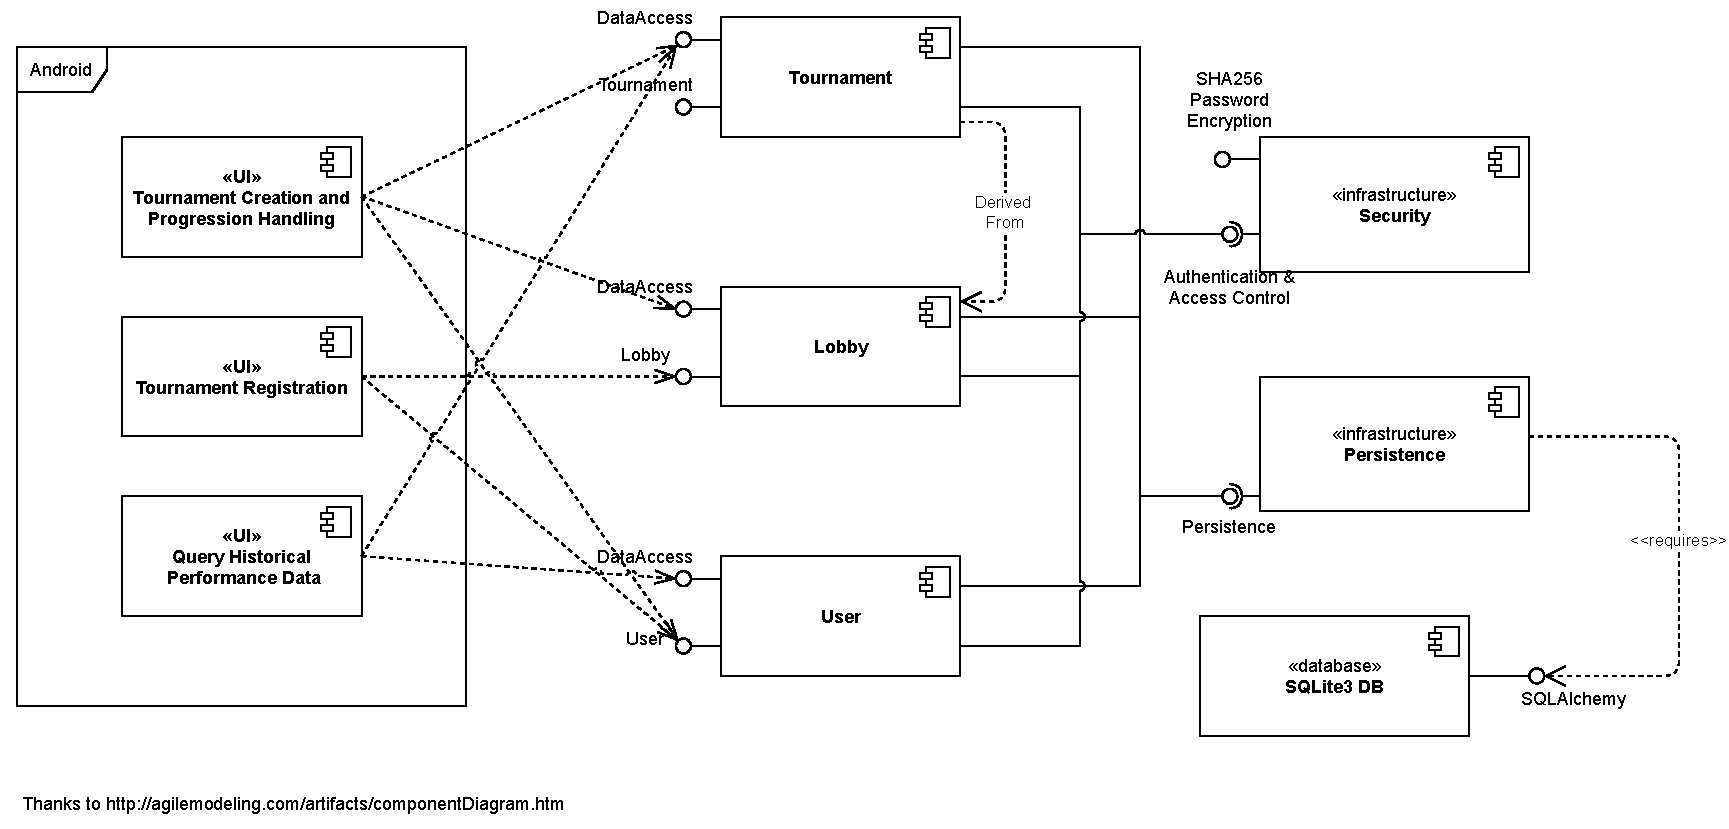
\includegraphics[width=18.5cm]{../diagrams/component_diag.pdf}
        \caption{\texttt{Brackit - }\href{https://sparxsystems.com/resources/tutorials/uml2/index.html}{UML 2} Architectural Component Diagram}
        \end{figure}
\end{center}
\vfill

\clearpage
\subsubsection{ER Diagram}
\vfill
\begin{center}
    \begin{figure}[h]
        \centering
        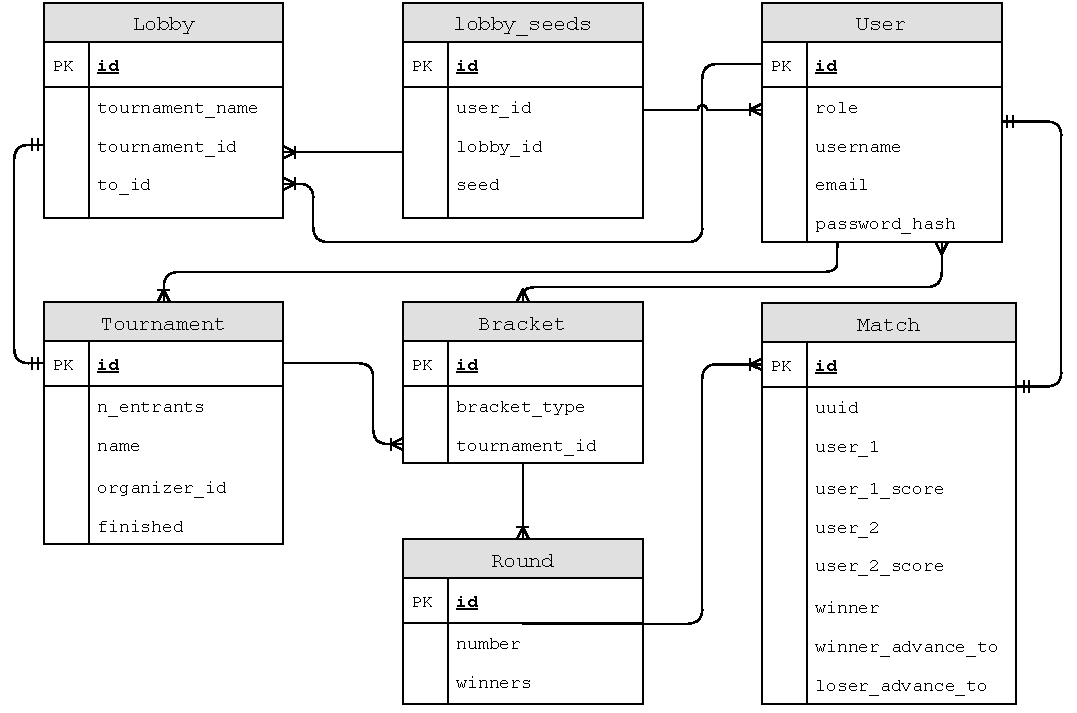
\includegraphics[width=18.5cm]{../diagrams/er_compressed.pdf}
        \caption{\texttt{Brackit - } Entity-Relationship (ER) Diagram}
        \end{figure}
\end{center}
\vfill
\clearpage
\section{Design}

\subsection{Description and Justification of Design Patterns}
\begin{enumerate}
    \item \textit{Facade}
    
    The Facade pattern intends to provide a unified interface to a set of interfaces in a subsystem. 
    For our backend, the API endpoints contained in the \href{https://github.com/alextrosta/brackit/blob/master/backend/app/routes.py}{\texttt{routes}} module constitute our Facade. Each endpoint provides a URL which the user can access
    to invoke all necessary interfaces to execute the necessary code in the backend.

    This pattern provides a singular hub through which frontend clients can access backend data.
    Modelling our server as a Facade centralized all exposed endpoints and allowed for ease of use and extensibility.

    \item \textit{Singleton} 
    
    The Singleton pattern intends to ensure a class has only one instance and to allow global 
    access to that class. The \texttt{Flask} app object leverages the Singleton pattern in its design. It is instantiated only once (when the server is started), and is globally accessible. \\
    A Singleton design pattern for the app object is an appropriate choice because when the app class is instantiated, it acts as a representation of the \texttt{Flask} server at compile-time.
    % The justification for the use of the Singleton pattern for the app object is because the app 
    % class itself, when instantiated, is the representation of the Flask server instance at compile-time,
    This representation encapsulates all current server modifications and customizations 
    and specifies the database schema, API endpoints, as well as any backend refactoring. 
    Correspondingly, this guarantees that the app is only instantiated once. This maintains consistency throughout a session and mitigates the possibility that multiple clients create  duplicate endpoints, which would result in unintentional behaviour such as inconsistent method invocations.
\end{enumerate}

\subsection{Frontend Frameworks Rationalization}
% The first decision we made at the planning stage was to decide the platform for our app.
To develop our mobile application, both Android and iOS platforms could have met our needs.
iOS was a strong candidate since it has a large market audience and it would have allowed us to build the app in a fast and easy way. The disadvantage is that we are more restricted with writing Swift code and building up components for specific devices.
Developing using Android allows for more flexible feature implementation using an open source platform that could be adapted to cater to the specific needs of \texttt{Brackit}.
The downside is that developing Android apps could be more complex since there is no standardization for devices and components. \\
We decided to proceed with Android since more team members are comfortable with the Android environment. This gave us the flexibility to run an Android environment on both Mac iOS and Windows operating systems.
For Frontend development, we used Kotlin to integrate with Android Studio. Although Java seems to be a popular choice for Android app developers, Kotlin, as a relatively new open source language, has been gaining popularity for several reasons.
Kotlin is based on the JVM (Java Virtual Machine) and it is fully interoperable with Java. It can be seamlessly integrated with Android Studio. And, Kotlin is more lightweight than Java and can therefore significantly reduce the overhead associated with the project.

\subsection{Implementation Analysis}


    The \texttt{Brackit} backend was designed primarily to marry extensibility with the correctness of 
our relatively complex domain. The main challenge of the backend's design is the creation of 
correct brackets, as well as the maintenance of brackets as they progress to completion.
When a user creates a Tournament, \texttt{Brackit} initializes a \href{https://github.com/alextrosta/brackit/blob/master/backend/tournament.py#L18}{\texttt{tournament} object} in the backend, which itself creates
the \href{https://github.com/alextrosta/brackit/blob/master/backend/tournament.py#L59}{\texttt{bracket} objects}. Depending on the bracket type, the appropriate number of rounds are created, 
with each round containing the corresponding number of matches. This is handled automatically because
the number of rounds is determined by the number of entrants and the type of bracket (See Section \ref{sssec:ooas}).\\
Our backend uses the \href{https://flask.palletsprojects.com/en/1.1.x/}{\texttt{Flask}} python package to expose our bracket and user information to 
the frontend, as well as \href{https://www.sqlalchemy.org/}{SQLAlchemy} to manage this information in the database. SQLAlchemy provides a \href{https://flask-sqlalchemy.palletsprojects.com/en/2.x/models/}{\texttt{Model}} base-class that allows us to declare the tournament objects as database tables and a runtime interface by which we interact with our \href{https://www.sqlite.org/index.html}{\texttt{SQLite3}} database. We model each class in our class diagram in the \href{https://github.com/alextrosta/brackit/blob/master/backend/app/models.py}{\texttt{models}} module, which creates 
tables for each class and defines the table relationships in an object-oriented style. This 
allows us to easily and safely query the database when invoking APIs and enables 
retrieval of the specific object being requested. Additionally, these models allow for 
seamless SQL querying for user data, such as users' cross-tournament wins and losses. 

\subsection{Integration and Coupling Challenges}
As a consequence of utilizing SQLAlchemy model our classes in the database, we produced three 
layers of abstraction in our application: 
\begin{itemize}
    \item{the \texttt{Routes} layer, i.e. our API Facade, }
    \item{the \texttt{Model} layer, and}
    \item{the \texttt{Backend}
    layer, where bracket generation and progression handling logic is stored.}
\end{itemize}  This created some significant
challenges when designing for decoupling. When we query tables for requested objects in the \texttt{Routes} layer, 
we return the \texttt{Model} objects and not the \texttt{Backend} objects. Accessing \texttt{Backend} objects
after instantiation in the \texttt{Routes} layer became a significant challenge. We addressed this by moving the logic for inputting
match results directly into the \texttt{Model} layer, as that is the layer responsible for the representation of the objects 
in the database. \\
Also, we experimented with each class in the \texttt{Model} layer containing its corresponding \texttt{Backend} object 
as an attribute. However, because the \texttt{Tournament} object in the \texttt{Backend} instantiates its child objects such as the \texttt{Bracket}, 
\texttt{Rounds}, and \texttt{Matches} during initialization, it became impossible to map one to the other.
% This problem would be another area of future evolution for our system.
\\The final challenge we'll discuss relates to the encapsulation of user data within match objects (i.e. handling how matches ``know'' which entrants are participating in said matches). This is known as progression handling. For matches in the initial rounds, progression handling and placement are trivial since 
the entrants are placed into the matches in the first round when the Tournament is instantiated. However, as the tournament progresses, the client must POST win, loss, and progression data to the backend.
When the results of a match are reported, \texttt{Brackit} must determine where the winner and loser progress to. \\
To address this, we explored the use of pointers that correspond to each entrant in subsequent matches. 
% Each pointer % points to the winner attribute of the previous match which progresses to the subsequent match. 
However, 
% this 
% solution ran into problems with the SQLAlchemy model,
% as 
it became challenging to ensure that as the tournament 
progressed and pointers were instantiated with user data, the database reflected these changes. 
Ultimately, we decided to store references to two other match objects within a \texttt{Match} (\texttt{loserPlaysInMatch} and \texttt{winnerPlaysInMatch}). These attributes reference the matches that the loser and winner progress to. This approach simplified database 
representation and enabled intuitive bracket navigation on the frontend. That is, by inspecting a match's attributes, one could find subsequent matches in the tournament.
%  to find subsequent matches given a previous match, since one could find subsequent matches
% from a previous match just by inspecting that match object's attributes.


\subsection{Suggestions for Future Work}
\label{ssec:fw}

So far, \texttt{Brackit} only supports double elimination brackets, but this can be expanded by the addition of special cases in the \texttt{Bracket} constructor. An alternative approach would be to create an abstract \texttt{Bracket}
class with each bracket type as an extension of the abstract \texttt{Bracket} class. This may allow for 
code that is readable and iterable and would be worth the refactoring time if this project were 
to be expanded. \\
We also plan to streamline user entry to tournaments via their pre-registered \texttt{Brackit} accounts using a QR code for a given tournament that, when read, automatically enters the user into the tournament lobby. Our choices of  
the Facade Design pattern coupled with our Object-Oriented and Server-Client Architecture will facilitate the integration of this new feature. Specifically, by modelling a Tournament as an object, we can add an additional \href{https://docs.python.org/3/library/uuid.html}{\texttt{uuid}}
attribute that enables unique QR code generation and matching. Once this feature is supported, further frontend functionality will be needed to display a QR code from the 
\texttt{/api/lobby/<int:lobby\_id>/add-user/} endpoint, as well QR Code recognition from an additional API endpoint.






\clearpage
\subsection{Design Diagrams}
\subsubsection{Backend UML Class Diagram}
\begin{center}
    \begin{figure}[htp]
        \centering
        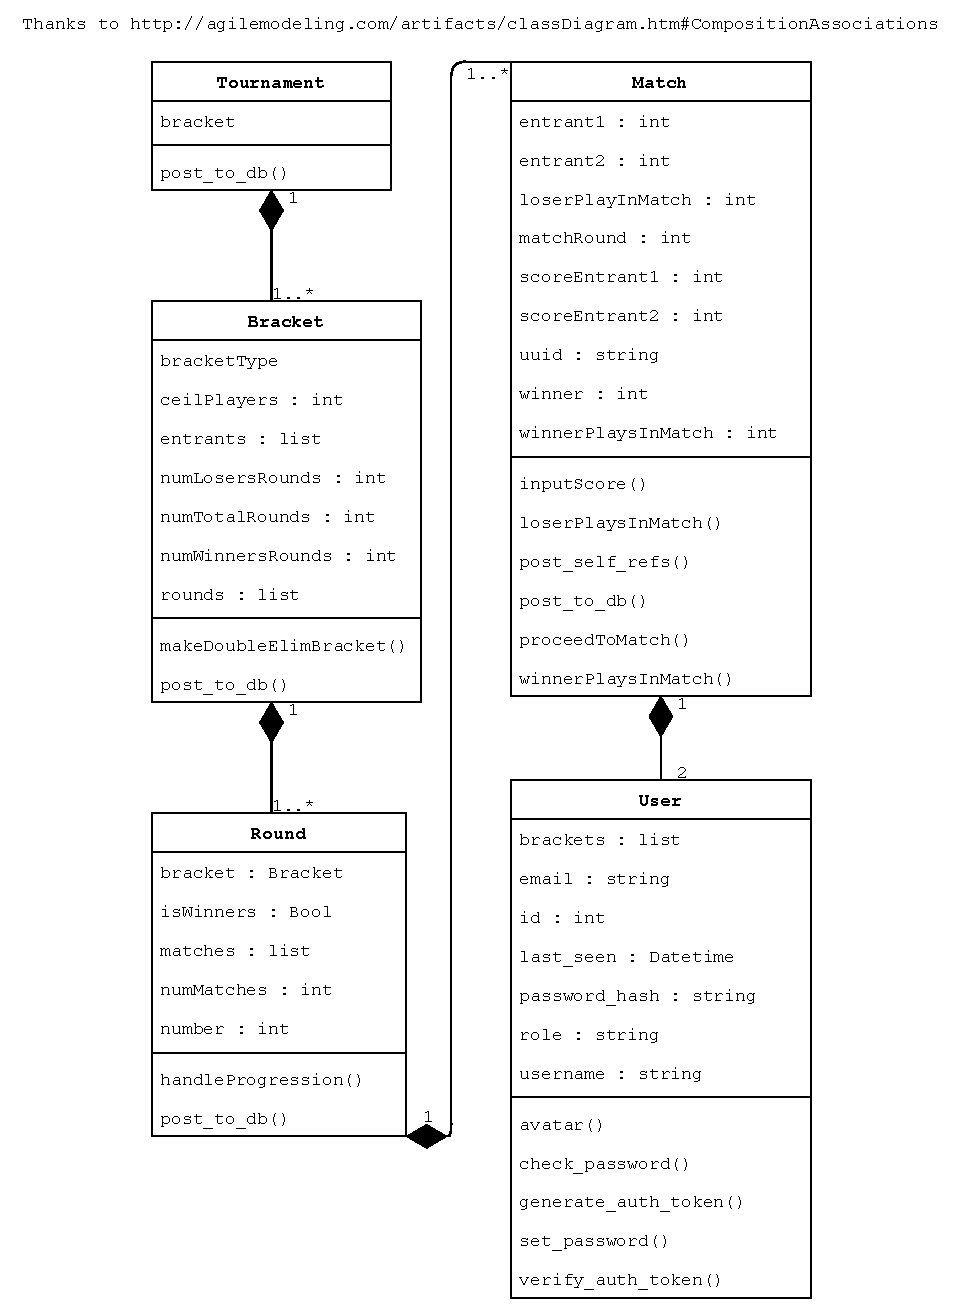
\includegraphics[width=13cm]{../diagrams/uml_class_tourn.pdf}
        \caption{\texttt{Brackit - } Backend UML Class Diagram}
        \end{figure}
\end{center}
\clearpage
\subsubsection{Frontend UML Class Diagram}
\begin{center}
    \begin{figure}[htp]
        \centering
        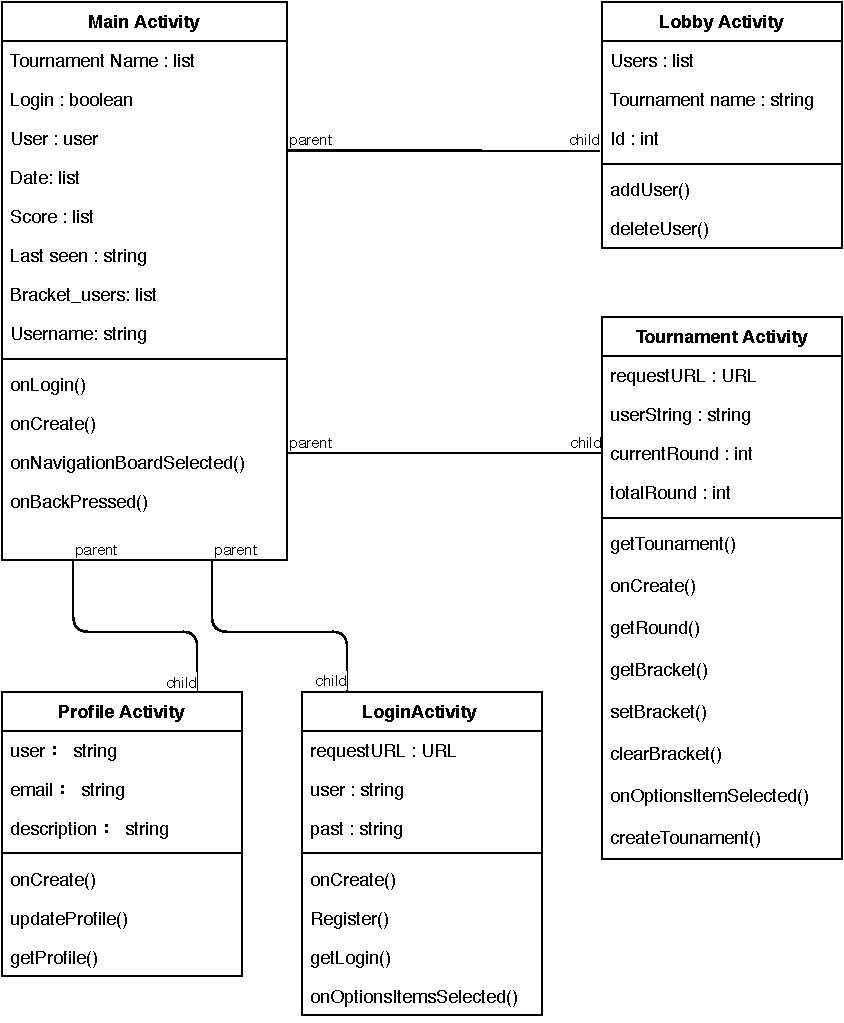
\includegraphics[width=9cm]{../diagrams/brackit-frontend-classDiagram.pdf}
        \caption{\texttt{Brackit - } Frontend UML Class Diagram}
        \end{figure}
\end{center}
\subsubsection{\texttt{Create Tournament} Sequence Diagram}
% \vfill
\begin{center}
    \begin{figure}[htp]
        \centering
        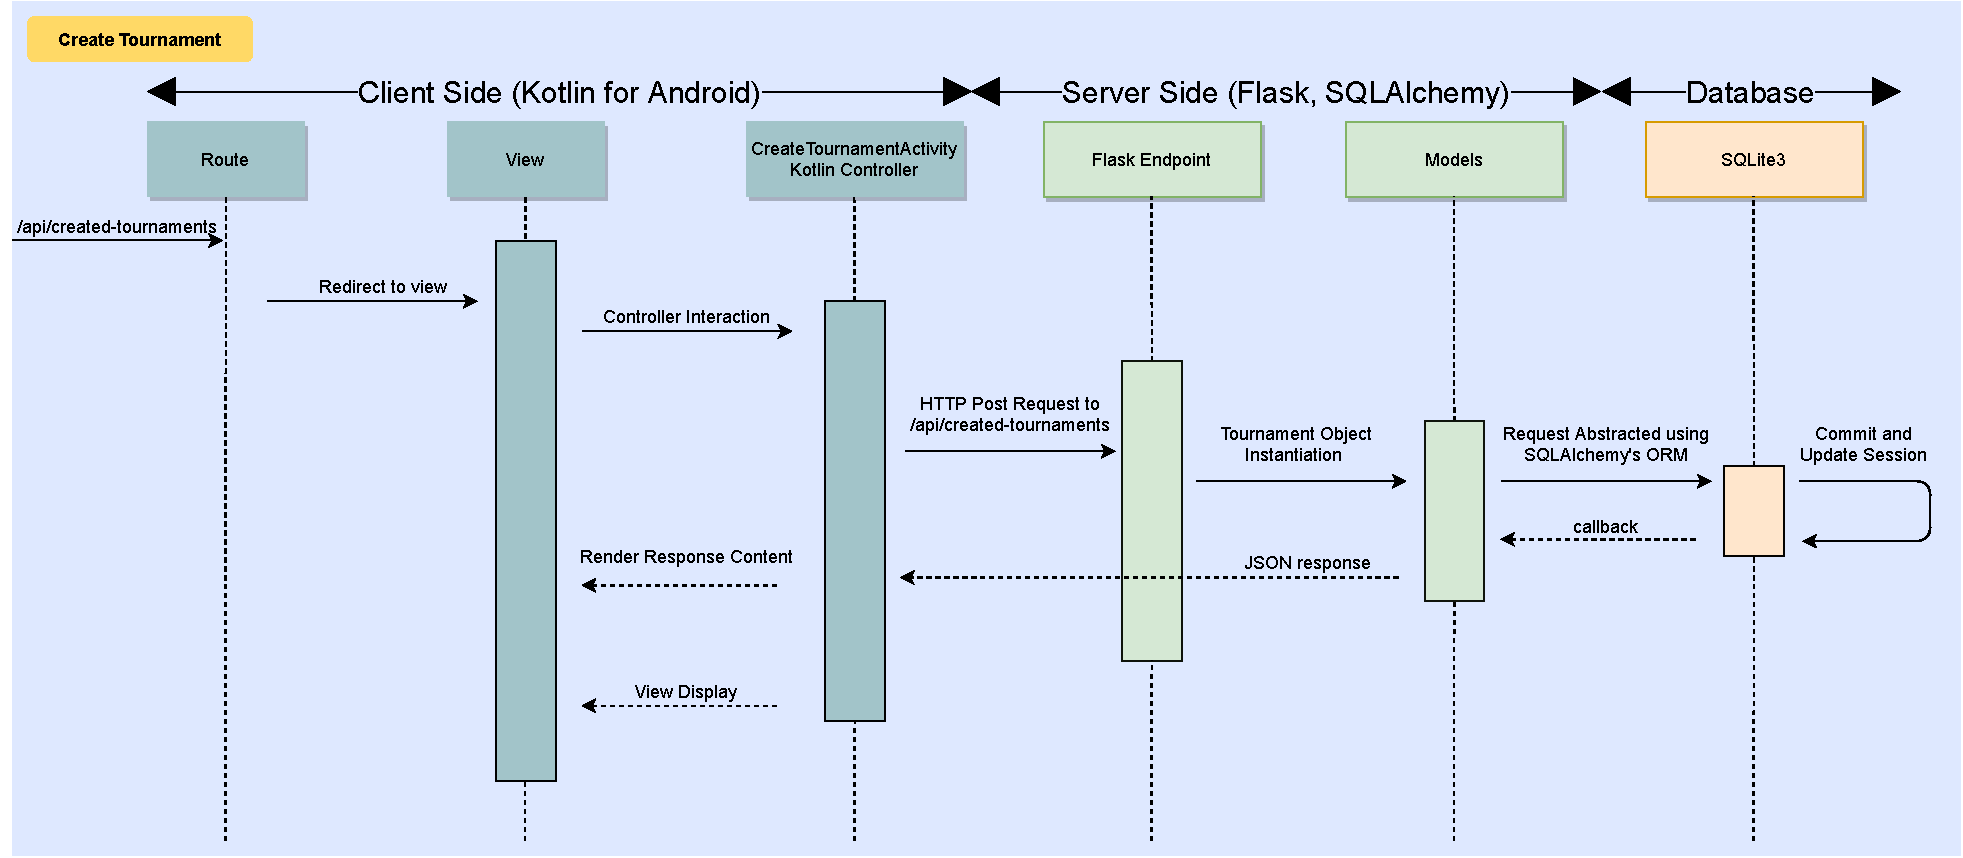
\includegraphics[width=10cm]{../diagrams/sequence.pdf}
        \caption{\texttt{Brackit: Create Tournament} Sequence Diagram}
        \end{figure}
\end{center}
% \vfill

\clearpage
\section{Assignment of Tasks}
\begin{itemize}
    \item{Jaime Herzog, 101009321: 
        \begin{itemize}
            \item{Report: 
                \begin{itemize}
                    \item{Sections 2.1, 2.3 - 2.5}
                \end{itemize}
            }
            \item{\texttt{Brackit}: 
                \begin{itemize}
                    \item{\texttt{Backend} Layer}
                    \item{Algorithm for generation of double elimination brackets}
                    \item{Progression Handling}
                    \item{\texttt{winsAndLosses} endpoint - Performance Metrics Endpoint}
                \end{itemize}
            }
        \end{itemize}
    }
    \item{Suohong Liu, 101002340:
    \begin{itemize}
        \item{Report:
            \begin{itemize}
                \item{}
            \end{itemize}
        }
        \item{\texttt{Brackit}:
            \begin{itemize}
                \item{Asynchronous information processing with the server}
                \item{Progression handling - frontend implementation}
                \item{Endpoint testing}
            \end{itemize}
        }
    \end{itemize}
    }
    \item{Xiyi Liu, 101004577:
        \begin{itemize}
            \item{Report:
                \begin{itemize}
                    \item{Section 2.2}
                    \item{Figure 5}
                \end{itemize}
            }
            \item{\texttt{Brackit}:
                \begin{itemize}
                    \item{User interface design for frontend}
                    \item{Endpoints testing}
                    \item{Implementation of user activities}
                \end{itemize}
            }
        \end{itemize}
    }
    \item{Alex Trostanovsky, 100984702: 
        \begin{itemize}
            \item{Report: 
                \begin{itemize}
                    \item{\LaTeX Compilation}
                    \item{Figures 1-4, 6}
                    \item{Sections 1.1-1.2}
                \end{itemize}
            }
            \item{\texttt{Brackit}: 
                \begin{itemize}
                    \item{\texttt{Models}, \texttt{Routes} Layers}
                    \item{SQLite3 Database Initialization, Migration}
                    \item{Mock data population scripts}
                    \item{Endpoints testing and implementation}
                \end{itemize}
            }    
        \end{itemize}
    }
    
\end{itemize}

\clearpage
% \cite{wiki:xxx}
\bibliographystyle{unsrt}
\bibliography{ref.bib}


\end{document}